\chapter{実験}\label{zikken.tex}
我々の研究グループでは安全運転支援システムの構築を目指す.
システムの構築には運転行動の解析に加えて,ドライバが置かれている状況も併せて考える必要がある.
本論文では,まずサポートベクターマシンを用いた運転シーン分類における運転シーンのBoK特徴量の有効性について検証するため,運転シーンを交差点一時停止前,一時停止後の2シーンに分類する実験を行う.
次に,運転シーンを道路上に自動車等が存在する状態と存在しない状態の2シーンに分類する実験を行う.

\section{交差点一時停止前,一時停止後への分類実験}

\subsection{実験内容}
運転シーンのBoK特徴量を用いれば,何が可能で何が不可能であるかを明確にするため,運転シーンの2シーンへの分類を行う.\\

\subsection{定義}
見通しの悪い無信号の交差点を対象とし,交差点進入前の一時停止の標識から停止線までを一時停止,動き出してから曲がりきるまでを一時停止後と定義する(図\ref{fig:teigi}参照).

\begin{figure}[htbp]
  \begin{center}
    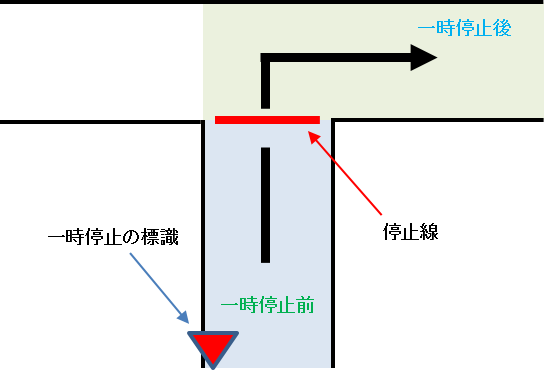
\includegraphics[clip,width=8.0cm]{./images/teigi.png}
    \caption{定義}
    \label{fig:teigi}
  \end{center}
\end{figure}

\subsection{解析対象データ}
ドライビングシミュレータデータセットの内,一周目の交差点1,2,3の画像を用いて実験を行う.
それぞれの交差点の一時停止前,一時停止後の画像枚数を統一するため,交差点1はそれぞれ等間隔で70枚,交差点2は100枚,交差点3は100枚抜粋した画像を使用する(図
\ref{fig:experimentaldata1}参照).\\

\begin{figure}[htbp]
  \begin{center}
    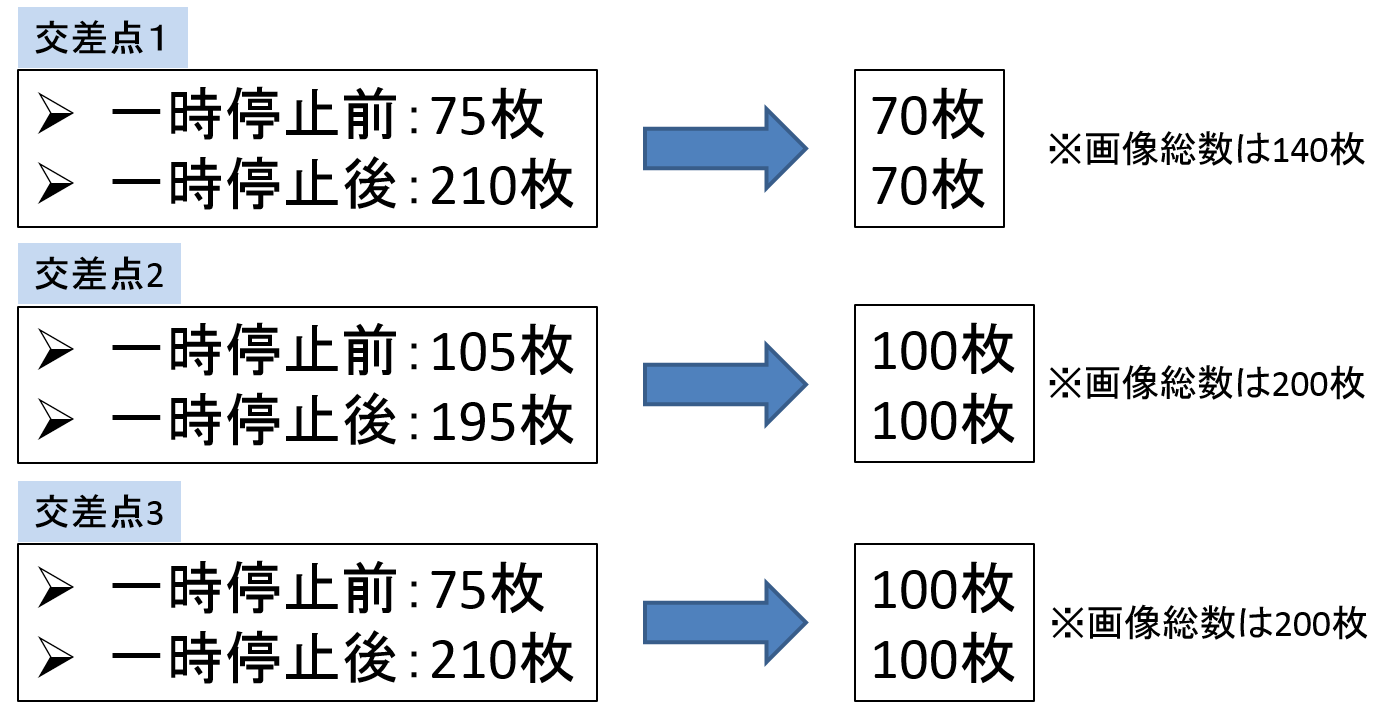
\includegraphics[clip,width=8.0cm]{./images/experimentaldata1.png}
    \caption{解析対象データ}
    \label{fig:experimentaldata1}
  \end{center}
\end{figure}

\subsection*{各交差点の画像例}
各交差点1,2,3の一時停止前,一時停止後の画像例を記す(図\ref{fig:ds1stop1}から図\ref{fig:ds3turn4}参照).
    
\begin{figure}[htbp]
  \begin{center}
    \begin{tabular}{cc}
      % 1
      \begin{minipage}{0.5\hsize}
        \begin{center}
          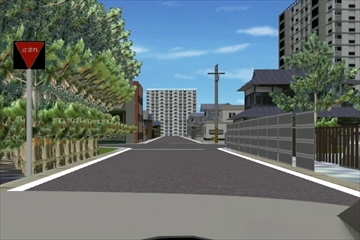
\includegraphics[clip, width=8.0cm]{./images/ds1stop001.png}
          \caption{交差点1:一時停止前1}
           \label{fig:ds1stop1}
        \end{center}           
      \end{minipage}
      % 2
      \begin{minipage}{0.5\hsize}
        \begin{center}
          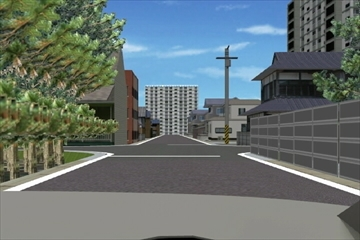
\includegraphics[clip, width=8.0cm]{./images/ds1stop023.png}
          \caption{交差点1:一時停止前2}
         \label{fig:ds1stop2}
        \end{center}
      \end{minipage}
    \end{tabular}
  \end{center}
\end{figure}

\begin{figure}[htbp]
  \begin{center}
    \begin{tabular}{cc}
      % 1
      \begin{minipage}{0.5\hsize}
        \begin{center}
          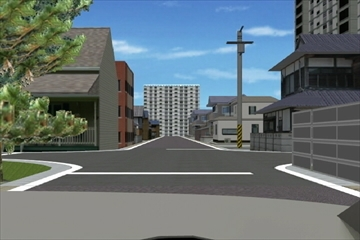
\includegraphics[clip, width=8.0cm]{./images/ds1stop046.png}
          \caption{交差点1:一時停止前3}
         \label{fig:ds1stop3}
        \end{center}
      \end{minipage}
      % 2
      \begin{minipage}{0.5\hsize}
        \begin{center}
          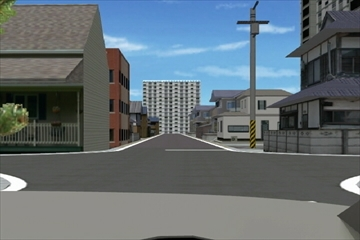
\includegraphics[clip, width=8.0cm]{./images/ds1stop069.png}
          \caption{交差点1:一時停止前4}
        \end{center}
      \end{minipage}
     \label{fig:ds1stop4}
    \end{tabular}
  \end{center}
\end{figure}



\begin{figure}[htbp]
  \begin{center}
    \begin{tabular}{cc}
      % 1
      \begin{minipage}{0.5\hsize}
        \begin{center}
          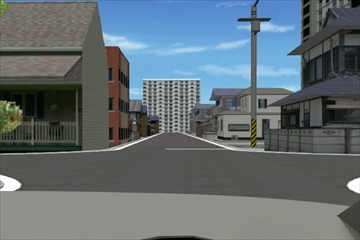
\includegraphics[clip, width=8.0cm]{./images/ds1turn001.png}
          \caption{交差点1:一時停止後1}
         \label{fig:ds1turn1}
        \end{center}          
      \end{minipage}
      % 2
      \begin{minipage}{0.5\hsize}
        \begin{center}
          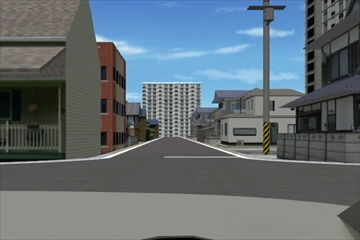
\includegraphics[clip, width=8.0cm]{./images/ds1turn023.png}
          \caption{交差点1:一時停止後2}
         \label{fig:ds1turn2}
        \end{center}
      \end{minipage}
    \end{tabular}
  \end{center}
\end{figure}

\begin{figure}[htbp]
  \begin{center}
    \begin{tabular}{cc}
      % 1
      \begin{minipage}{0.5\hsize}
        \begin{center}
          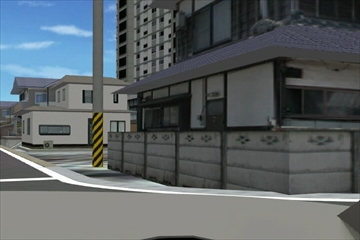
\includegraphics[clip, width=8.0cm]{./images/ds1turn046.png}
          \caption{交差点1:一時停止後3}
         \label{fig:ds1turn3}
        \end{center}
      \end{minipage}
      % 2
      \begin{minipage}{0.5\hsize}
        \begin{center}
          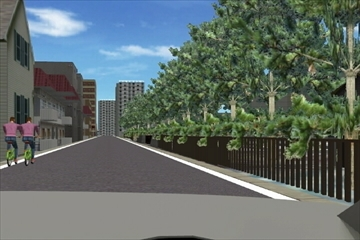
\includegraphics[clip, width=8.0cm]{./images/ds1turn069.png}
          \caption{交差点1:一時停止後4}
         \label{fig:ds1turn4}
        \end{center}
      \end{minipage}
    \end{tabular}
  \end{center}
\end{figure}


\begin{figure}[htbp]
  \begin{center}
    \begin{tabular}{cc}
      % 1
      \begin{minipage}{0.5\hsize}
        \begin{center}
          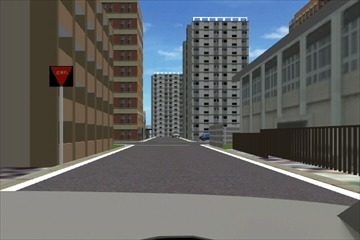
\includegraphics[clip, width=8.0cm]{./images/ds2stop001.png}
          \caption{交差点2:一時停止前1}
         \label{fig:ds2stop1}
        \end{center}
      \end{minipage}
      % 2
      \begin{minipage}{0.5\hsize}
        \begin{center}
          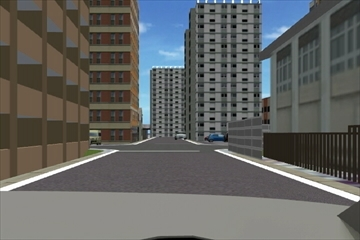
\includegraphics[clip, width=8.0cm]{./images/ds2stop033.png}
          \caption{交差点2:一時停止前2}
         \label{fig:ds2stop2}
        \end{center}
      \end{minipage}
    \end{tabular}
  \end{center}
\end{figure}

\begin{figure}[htbp]
  \begin{center}
    \begin{tabular}{cc}
      % 1
      \begin{minipage}{0.5\hsize}
        \begin{center}
          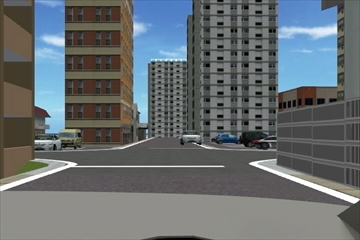
\includegraphics[clip, width=8.0cm]{./images/ds2stop066.png}
          \caption{交差点2:一時停止前3}
         \label{fig:ds2stop3}
        \end{center}
      \end{minipage}
      % 2
      \begin{minipage}{0.5\hsize}
        \begin{center}
          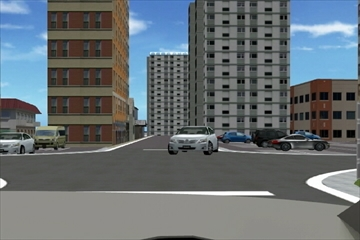
\includegraphics[clip, width=8.0cm]{./images/ds2stop099.png}
          \caption{交差点2:一時停止前4}
         \label{fig:ds2stop4}
        \end{center}
      \end{minipage}
    \end{tabular}
  \end{center}
\end{figure}


\begin{figure}[htbp]
  \begin{center}
    \begin{tabular}{cc}
      % 1
      \begin{minipage}{0.5\hsize}
        \begin{center}
          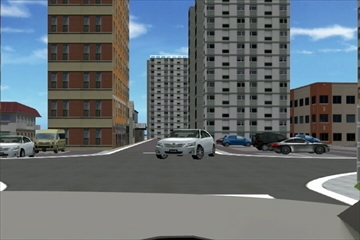
\includegraphics[clip, width=8.0cm]{./images/ds2turn001.png}
          \caption{交差点2:一時停止後1}
         \label{fig:ds2turn1}
        \end{center}
      \end{minipage}
      % 2
      \begin{minipage}{0.5\hsize}
        \begin{center}
          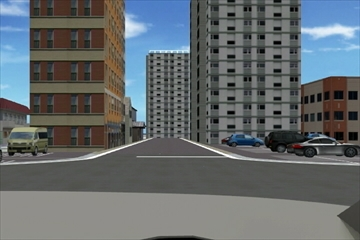
\includegraphics[clip, width=8.0cm]{./images/ds2turn033.png}
          \caption{交差点2:一時停止後2}
         \label{fig:ds2turn2}
        \end{center}
      \end{minipage}
    \end{tabular}
  \end{center}
\end{figure}

\begin{figure}[htbp]
  \begin{center}
    \begin{tabular}{cc}
      % 1
      \begin{minipage}{0.5\hsize}
        \begin{center}
          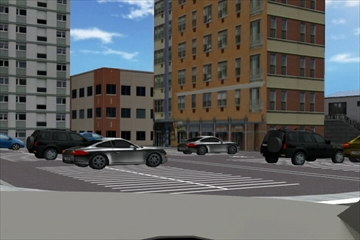
\includegraphics[clip, width=8.0cm]{./images/ds2turn066.png}
          \caption{交差点2:一時停止後3}
         \label{fig:ds2turn3}
        \end{center}
      \end{minipage}
      % 2
      \begin{minipage}{0.5\hsize}
        \begin{center}
          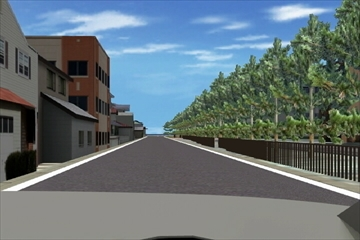
\includegraphics[clip, width=8.0cm]{./images/ds2turn099.png}
          \caption{交差点2:一時停止後4}
         \label{fig:ds2turn4}
        \end{center}
      \end{minipage}
    \end{tabular}
  \end{center}
\end{figure}



\begin{figure}[htbp]
  \begin{center}
    \begin{tabular}{cc}
      % 1
      \begin{minipage}{0.5\hsize}
        \begin{center}
          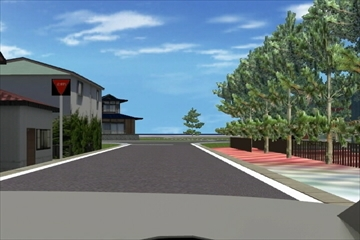
\includegraphics[clip, width=8.0cm]{./images/ds3stop001.png}
          \caption{交差点3:一時停止前1}
         \label{fig:ds3stop1}
        \end{center}
      \end{minipage}
      % 2
      \begin{minipage}{0.5\hsize}
        \begin{center}
          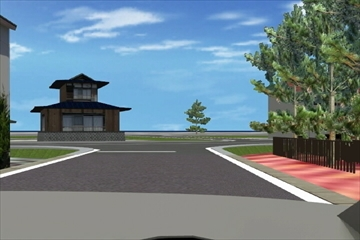
\includegraphics[clip, width=8.0cm]{./images/ds3stop033.png}
          \caption{交差点3:一時停止前2}
         \label{fig:ds3stop2}
        \end{center}
      \end{minipage}
    \end{tabular}
  \end{center}
\end{figure}

\begin{figure}[htbp]
  \begin{center}
    \begin{tabular}{cc}
      % 1
      \begin{minipage}{0.5\hsize}
        \begin{center}
          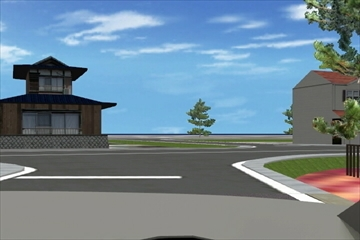
\includegraphics[clip, width=8.0cm]{./images/ds3stop066.png}
          \caption{交差点3:一時停止前3}
         \label{fig:ds3stop3}
        \end{center}
      \end{minipage}
      % 2
      \begin{minipage}{0.5\hsize}
        \begin{center}
          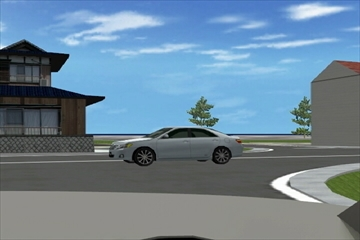
\includegraphics[clip, width=8.0cm]{./images/ds3stop099.png}
          \caption{交差点3:一時停止前4}
         \label{fig:ds3stop4}
        \end{center}
      \end{minipage}
    \end{tabular}
  \end{center}
\end{figure}


\begin{figure}[htbp]
  \begin{center}
    \begin{tabular}{cc}
      % 1
      \begin{minipage}{0.5\hsize}
        \begin{center}
          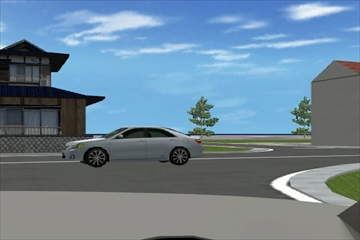
\includegraphics[clip, width=8.0cm]{./images/ds3turn001.png}
          \caption{交差点3:一時停止後1}
         \label{fig:ds3turn1}
        \end{center}
      \end{minipage}
      % 2
      \begin{minipage}{0.5\hsize}
        \begin{center}
          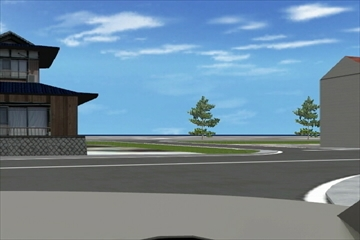
\includegraphics[clip, width=8.0cm]{./images/ds3turn033.png}
          \caption{交差点3:一時停止後2}
         \label{fig:ds3turn2}
        \end{center}
      \end{minipage}
    \end{tabular}
  \end{center}
\end{figure}

\begin{figure}[htbp]
  \begin{center}
    \begin{tabular}{cc}
      % 1
      \begin{minipage}{0.5\hsize}
        \begin{center}
          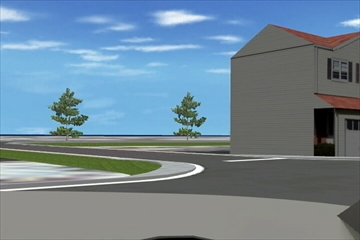
\includegraphics[clip, width=8.0cm]{./images/ds3turn066.png}
          \caption{交差点3:一時停止後3}
         \label{fig:ds3turn3}
        \end{center}
      \end{minipage}
      % 2
      \begin{minipage}{0.5\hsize}
        \begin{center}
          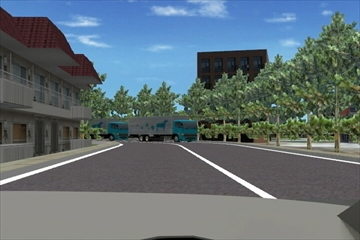
\includegraphics[clip, width=8.0cm]{./images/ds3turn099.png}
          \caption{交差点3:一時停止後4}
         \label{fig:ds3turn4}
        \end{center}
      \end{minipage}
    \end{tabular}
  \end{center}
\end{figure}

\newpage
\subsection{実験方法}
各交差点の一時停止前,一時停止後の両画像を学習データ,テストデータとして使用した分類実験を行う.
なお,画像からBoK特徴量を生成する際は,SIFTによるGridとSURFによるSparseの二つの方法で行う.行った実験を下の表\ref{tb:experiment1-1}と表\ref{tb:experiment1-2}に示す.\\

\begin{table}[htbp]
  \begin{center}
    \caption{行った実験1-1}
    \begin{tabular}{|c||c|c|c|c|} \hline
      & 対象交差点 & 特徴量生成手法 & 学習データ & テストデータ \\ \hline \hline
      実験1 & 交差点1 & SIFT(Grid) & 各奇数番目(計70枚) & 各偶数番目(計70枚) \\ \hline
      実験2 & 交差点2 & SIFT(Grid) & 各奇数番目(計100枚) & 各偶数番目(計100枚) \\ \hline
      実験3 & 交差点3 & SIFT(Grid) & 各奇数番目(計100枚) & 各偶数番目(計100枚) \\ \hline
      実験4 & 交差点1 & SURF(Sparse) & 各奇数番目(計70枚) & 各偶数番目(計70枚) \\ \hline
      実験5 & 交差点2 & SURF(Sparse) & 各奇数番目(計100枚) & 各偶数番目(計100枚) \\ \hline
      実験6 & 交差点3 & SURF(Sparse) & 各奇数番目(計100枚) & 各偶数番目(計100枚) \\ \hline
      \end{tabular}
    \label{tb:experiment1-1}
  \end{center}
\end{table}

\begin{table}[htbp]
  \begin{center}
    \caption{行った実験1-2}
    \begin{tabular}{|c||c|c|c|c|} \hline
      & 特徴量生成手法 & 学習データ & テストデータ \\ \hline \hline
      実験7 & SIFT(Grid) & 交差点2(200枚) & 交差点1 \\ 
       &  & 交差点3(200枚) & (計140枚) \\ \hline
      実験8 & SIFT(Grid) & 交差点1(200枚) & 交差点2 \\
       &  & 交差点3(200枚) & (計200枚) \\ \hline
      実験9 & SIFT(Grid) & 交差点1(140枚) & 交差点3 \\ 
       &  & 交差点2(200枚) & (計200枚) \\ \hline
      実験10 & SURF(Sparse) & 交差点2(200枚) & 交差点1 \\ 
       &  & 交差点3(200枚) & (計140枚) \\ \hline
      実験11 & SURF(Sparse) & 交差点1(200枚) & 交差点2 \\ 
       &  & 交差点3(200枚) & (計200枚) \\ \hline
      実験12 & SURF(Sparse) & 交差点1(140枚) & 交差点3 \\ 
       &  & 交差点2(200枚) & (計200枚) \\ \hline
      \end{tabular}
    \label{tb:experiment1-2}
  \end{center}
\end{table}

\newpage

\subsection{実験結果}
各実験結果を表に記す.\\

\subsubsection{実験1から6結果}
実験1から6までの結果を下の表\ref{tb:result1-1}に示す.
各実験とも誤識別が少なく,識別率が高かった.\\

\begin{table}[htbp]
  \begin{center}
    \caption{実験結果1-1}
    \begin{tabular}{|c||c|c|} \hline
      & 識別成功画像枚数 & 識別率 \\ \hline \hline
      実験1 & 69/70 & 98.57\% \\ \hline
      実験2 & 98/100 & 98.00\% \\ \hline
      実験3 & 97/100 & 97.00\% \\ \hline
      実験4 & 65/70 & 92.85\% \\ \hline
      実験5 & 93/100 & 93.00\% \\ \hline
      実験6 & 98/100 & 98.00\% \\ \hline
     \end{tabular}
   \label{tb:result1-1}
  \end{center}
\end{table}


\subsubsection*{誤分類データ}
実験1から実験6の各実験の中で,誤分類された画像を図\ref{fig:ds1turn44}から図に示す.\\

\subsubsection*{実験1での一時停止後の誤分類シーン}
実験1の中で一時停止前として誤分類された画像\\

\begin{figure}[htbp]
  \begin{center}
    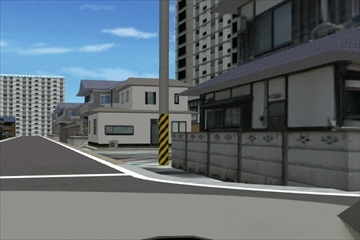
\includegraphics[clip,width=8.0cm]{./images/ds1turn044.png}
    \caption{交差点1:一時停止後44}
    \label{fig:ds1turn44}
  \end{center}
\end{figure}

図\ref{fig:ds1turn44}は一時停止後であるが一時停止前として分類された.\\


\subsubsection*{実験2での一時停止前の誤分類シーン}
実験2の中で一時停止後として誤分類された画像\\

\begin{figure}[htbp]
  \begin{center}
    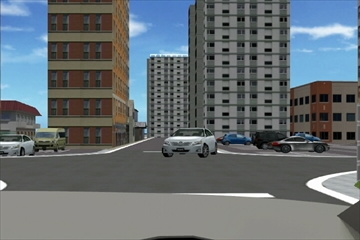
\includegraphics[clip,width=8.0cm]{./images/ds2stop100.png}
    \caption{交差点2:一時停止前100}
    \label{fig:ds2stop100}
  \end{center}
\end{figure}

図\ref{fig:ds2stop100}は一時停止前であるが一時停止後として分類された.\\


\subsubsection*{実験2での一時停止後の誤分類シーン}
実験2の中で一時停止前として誤分類された画像\\

\begin{figure}[htbp]
  \begin{center}
    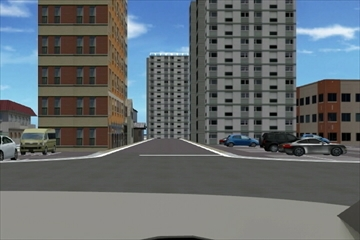
\includegraphics[clip,width=8.0cm]{./images/ds2turn026.png}
    \caption{交差点2:一時停止後26}
    \label{fig:ds2turn26}
  \end{center}
\end{figure}

図\ref{fig:ds2turn26}は一時停止後であるが一時停止前として分類された.\\


\subsubsection*{実験3での一時停止前の誤分類シーン}
実験3の中で一時停止後として誤分類された画像\\

\begin{figure}[htbp]
  \begin{center}
    \begin{tabular}{cc}
      % 1
      \begin{minipage}{0.5\hsize}
        \begin{center}
          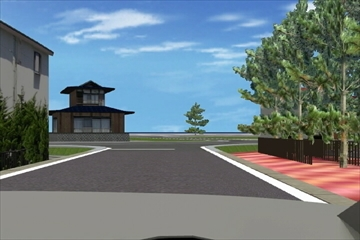
\includegraphics[clip, width=8.0cm]{./images/ds3stop024.png}
          \caption{交差点3:一時停止前24}
         \label{fig:ds3stop24}
        \end{center}
      \end{minipage}
      % 2
      \begin{minipage}{0.5\hsize}
        \begin{center}
          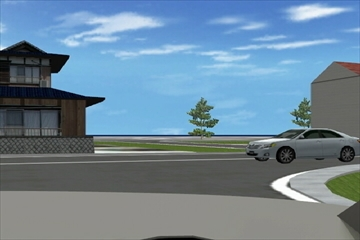
\includegraphics[clip, width=8.0cm]{./images/ds3stop094.png}
          \caption{交差点3:一時停止前94}
         \label{fig:ds3stop94}
        \end{center}
      \end{minipage}
    \end{tabular}
  \end{center}
\end{figure}

図\ref{fig:ds3stop24}と図\ref{fig:ds3stop94}は一時停止前であるが一時停止後として分類された.\\


\subsubsection*{実験3での一時停止後の誤分類シーン}
実験3の中で一時停止前として誤分類された画像\\

\begin{figure}[htbp]
  \begin{center}
    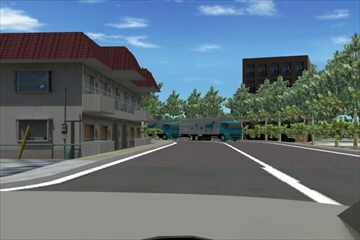
\includegraphics[clip,width=8.0cm]{./images/ds3turn088.png}
    \caption{交差点3:一時停止後88}
    \label{fig:ds3turn88}
  \end{center}
\end{figure}

図\ref{fig:ds3turn88}は一時停止後であるが一時停止前として分類された.\\


\subsubsection*{実験4での一時停止前の誤分類シーン}
実験4の中で一時停止後として誤分類された画像\\

\begin{figure}[htbp]
  \begin{center}
    \begin{tabular}{cc}
      % 1
      \begin{minipage}{0.5\hsize}
        \begin{center}
          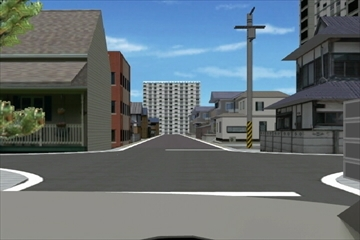
\includegraphics[clip, width=8.0cm]{./images/ds1stop062.png}
          \caption{交差点1:一時停止前62}
         \label{fig:ds1stop62}
        \end{center}
      \end{minipage}
      % 2
      \begin{minipage}{0.5\hsize}
        \begin{center}
          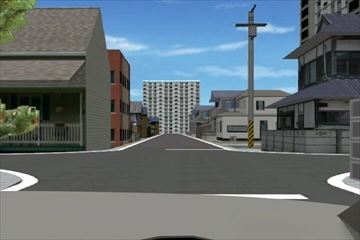
\includegraphics[clip, width=8.0cm]{./images/ds1stop064.png}
          \caption{交差点1:一時停止前64}
         \label{fig:ds1stop64}
        \end{center}
      \end{minipage}
    \end{tabular}
  \end{center}
\end{figure}

\begin{figure}[htbp]
  \begin{center}
    \begin{tabular}{ccc}
      % 1
      \begin{minipage}{0.5\hsize}
        \begin{center}
          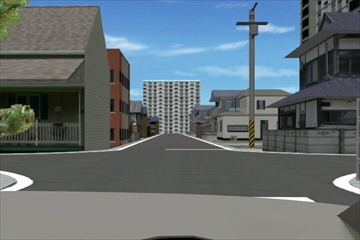
\includegraphics[clip, width=8.0cm]{./images/ds1stop066.png}
          \caption{交差点1:一時停止前66}
         \label{fig:ds1stop66}
        \end{center}
      \end{minipage}
      % 2
      \begin{minipage}{0.5\hsize}
        \begin{center}
          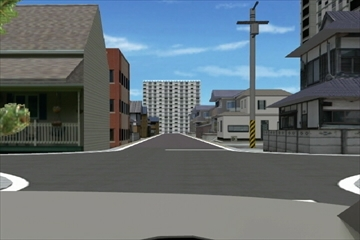
\includegraphics[clip, width=8.0cm]{./images/ds1stop068.png}
          \caption{交差点1:一時停止前68}
         \label{fig:ds1stop68}
        \end{center}
      \end{minipage}
    \end{tabular}
  \end{center}
\end{figure}]

\newpage

\begin{figure}[htbp]
  \begin{center}
    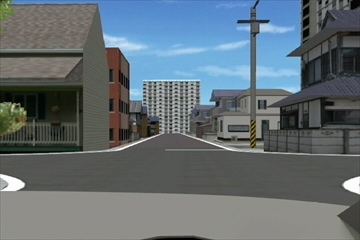
\includegraphics[clip,width=8.0cm]{./images/ds1stop070.png}
    \caption{交差点1:一時停止後70}
    \label{fig:ds1stop70}
  \end{center}
\end{figure}

図\ref{fig:ds1stop62}から図\ref{fig:ds1stop70}は一時停止前であるが一時停止後として分類された.\\

\subsubsection*{実験5での一時停止前の誤分類シーン}
実験2の中で一時停止後として誤分類された画像\\

\begin{figure}[htbp]
  \begin{center}
    \begin{tabular}{cc}
      % 1
      \begin{minipage}{0.5\hsize}
        \begin{center}
          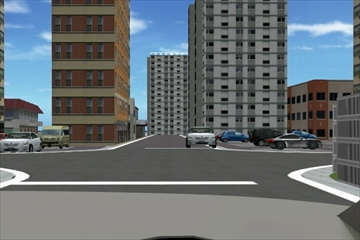
\includegraphics[clip, width=8.0cm]{./images/ds2stop084.png}
          \caption{交差点2:一時停止前84}
         \label{fig:ds2stop84}
        \end{center}
      \end{minipage}
      % 2
      \begin{minipage}{0.5\hsize}
        \begin{center}
          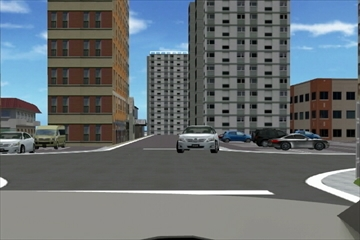
\includegraphics[clip, width=8.0cm]{./images/ds2stop096.png}
          \caption{交差点2:一時停止前96}
         \label{fig:ds2stop96}
        \end{center}
      \end{minipage}
    \end{tabular}
  \end{center}
\end{figure}

\newpage

\begin{figure}[htbp]
  \begin{center}
    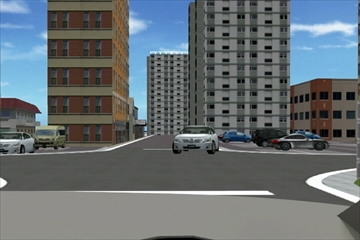
\includegraphics[clip,width=8.0cm]{./images/ds2stop098.png}
    \caption{交差点2:一時停止前98}
    \label{fig:ds2stop98}
  \end{center}
\end{figure}

図\ref{fig:ds2stop84}から図\ref{fig:ds2stop98}は一時停止前であるが一時停止後として分類された.\\



\subsubsection*{実験5での一時停止後の誤分類シーン}
実験2の中で一時停止前として誤分類された画像\\

\begin{figure}[htbp]
  \begin{center}
    \begin{tabular}{cc}
      % 1
      \begin{minipage}{0.5\hsize}
        \begin{center}
          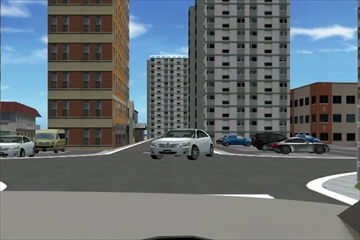
\includegraphics[clip, width=8.0cm]{./images/ds2turn002.png}
          \caption{交差点2:一時停止後2}
         \label{fig:ds2turn2}
        \end{center}
      \end{minipage}
      % 2
      \begin{minipage}{0.5\hsize}
        \begin{center}
          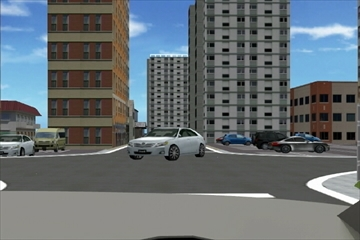
\includegraphics[clip, width=8.0cm]{./images/ds2turn004.png}
          \caption{交差点2:一時停止後4}
         \label{fig:ds2turn4}
        \end{center}
      \end{minipage}
    \end{tabular}
  \end{center}
\end{figure}

\newpage

\begin{figure}[htbp]
  \begin{center}
    \begin{tabular}{cc}
      % 1
      \begin{minipage}{0.5\hsize}
        \begin{center}
          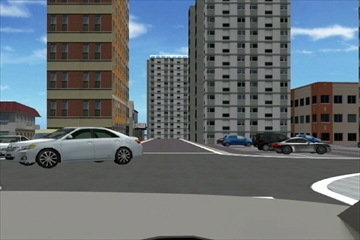
\includegraphics[clip, width=8.0cm]{./images/ds2turn012.png}
          \caption{交差点2:一時停止後12}
         \label{fig:ds2turn12}
        \end{center}
      \end{minipage}
      % 2
      \begin{minipage}{0.5\hsize}
        \begin{center}
          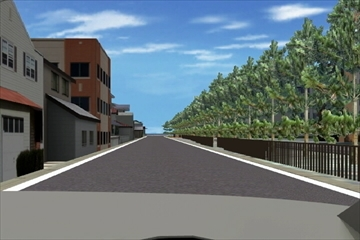
\includegraphics[clip, width=8.0cm]{./images/ds2turn096.png}
          \caption{交差点2:一時停止後96}
         \label{fig:ds2turn96}
        \end{center}
      \end{minipage}
    \end{tabular}
  \end{center}
\end{figure}

図\ref{fig:ds2turn2}から図\ref{fig:ds2turn96}は一時停止後であるが一時停止前として分類された.\\



\subsubsection*{実験6での一時停止前の誤分類シーン}
実験6の中で一時停止後として誤分類された画像\\

\begin{figure}[htbp]
  \begin{center}
    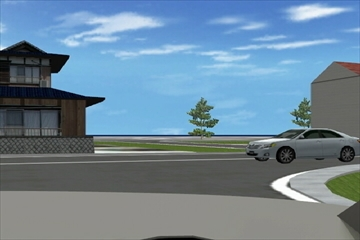
\includegraphics[clip,width=8.0cm]{./images/ds3stop094.png}
    \caption{交差点3:一時停止前94}
    \label{fig:ds3stop94}
  \end{center}
\end{figure}

図\ref{fig:ds3stop94}は一時停止前であるが一時停止後として分類された.\\


\newpage

\subsubsection*{実験6での一時停止後の誤分類シーン}
実験6の中で一時停止前として誤分類された画像\\

\begin{figure}[htbp]
  \begin{center}
    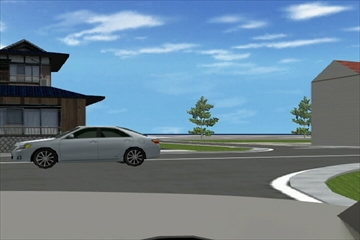
\includegraphics[clip,width=8.0cm]{./images/ds3turn002.png}
    \caption{交差点3:一時停止後2}
    \label{fig:ds3turn2}
  \end{center}
\end{figure}

図\ref{fig:ds3turn2}は一時停止後であるが一時停止前として分類された.\\


\subsubsection*{考察(実験1から6)}
実験1から6では,各交差点1から3のシーンに対してBoK特徴量とサポートベクターマシンを用いて一時停止前と一時停止後の2シーン分類を行った.
識別率は全て90%を越え,最も高い実験結果では98.57%で後分類シーン枚数が一枚という結果となった.
後分類されたシーンの多くは連続したシーンでかつ,一時停止前と一時停止後のシーンの境界部分であった.
これは視覚的にも似ているシーンであるため分類は困難であると考える.
シーンの境界部分ではなかった誤分類シーンは道路上に存在する白線や家,木々,電柱等の特徴量の影響を受け,誤分類されたと考えられる.
識別率が全体的に高い結果となった理由としては学習データとテストデータで用いたシーンが同じ交差点内のものであったためと考えられる.\\

\newpage

\subsubsection{実験7から12結果}
実験7から12までの結果を下の表\ref{tb:result1-2}に示す.\\

\begin{table}[htbp]
  \begin{center}
    \caption{実験結果1-2}
    \begin{tabular}{|c||c|c|c|} \hline
      & 識別成功画像枚数 & 識別率 & 平均識別率 \\ \hline \hline
      実験7 & 96/140 & 68.57\% & \\ \cline{1-3}
      実験8 & 100/200 & 50.00\% & 57.69\% \\ \cline{1-3}
      実験9 & 109/200 & 54.50\% & \\ \hline
      実験10 & 86/140 & 61.42\% & \\ \cline{1-3}
      実験11 & 124/200 & 62.00\% & 63.64\% \\ \cline{1-3}
      実験12 & 135/200 & 67.50\% & \\ \hline
     \end{tabular}
   \label{tb:result1-2}
  \end{center}
\end{table}

\subsubsection*{考察(実験7から12)}
実験7から12では,実験1から6と同様に各交差点1から3のシーンに対してBoK特徴量とサポートベクターマシンを用いて一時停止前と一時停止後の2シーン分類を行ったが,学習データとテストデータで用いるシーンは別々の交差点のシーンを用いた.
その結果,識別率は実験1から6と比較して全体的に悪くなった.
この事から,各交差点1から3のシーンから生成したBoK特徴量はあらゆるシーンに有効な特徴量ではなく,各交差点シーンに対応した特徴量である事が分かった.
ドライバの運転支援システムを想定し,この手法で高い識別率を維持する場合は膨大な学習データを必要とするため実用的ではない.
あらゆるシーンに有効な特徴量を見つけ出す必要があると考えられる.


\newpage

\section{道路上に自動車等が存在する状態と存在しない状態への分類実験}

\subsection{実験内容}
運転シーンを道路上に自動車等が存在する状態(以下:自動車)と存在しない状態(以下:その他)に分類し,道路上の特定物体の特徴が運転シーン分類に与える影響を解析した.\\

\subsection{解析対象データ}
ドライビングシミュレータセットの内,見通しの悪い無信号の交差点で車が横切るイベントが発生する一周目の交差点2,3,三周目の交差点1,2,3の画像を用いて実験を行う.それぞれの交差点の自動車,その他の画像枚数を統一するため,一周目の交差点2はそれぞれ等間隔で28枚,一周目の交差点3は17枚,三周目の交差点1は19枚,三周目の交差点2は15枚,三周目の交差点3は15枚抜粋した画像を使用する(図参照).\\

\begin{figure}[htbp]
  \begin{center}
    \includegraphics[clip,width=8.0cm]{./images/.png}
    \caption{交差点3:一時停止前94}
    \label{fig:ds3stop94}
  \end{center}
\end{figure}


\subsection{実験方法}

\subsection{実験結果}


